\section{Conclusões}
\label{conclusoes}

Nesta seção é feito o fechamento do trabalho, devendo ser descrito de forma sintética o problema abordado, a solução desenvolvida, como a solução foi validada, e quais os resultados e constatações mais significativas. No geral, a conclusão pode ser dividida em três partes: A (\textit{i}) conclusão (hipóteses foram comprovadas? qual foi o melhor método? etc), (\textit{ii}) contribuições e os (\textit{iii}) trabalhos futuros.

Uma dica é citar os objetivos do trabalho (geral e específicos) e descrever como fez para que fossem alcançados (ou não). Destaque a principal contribuição do trabalho, os pontos positivos e os negativos, associe evidências para cada conclusão que apresentar. 

Nos \textcolor{blue}{\textbf{Trabalhos Futuros}} é importante dar ao leitor uma noção das possibilidades de pesquisa que podem ser desenvolvidas a partir do que foi feito no seu trabalho. Isso aumenta as possibilidades do seu trabalho ser citado por outros autores.

Em relação as \textcolor{blue}{\textbf{Referências Bibliográficas}}, o ideal é organizar os artigos que baixar por ``\textit{ano, Sobrenome1ºautor - Título}'' de modo a evitar duplicidades. A ferramenta Mendeley \url{www.mendeley.com} é útil para organização de arquivos de referências (local ou nuvem), localização de conteúdo e para obtenção de referências no formato \LaTeX.

Inclua as  referências bibliográficas no arquivo  \textcolor{blue}{\textbf{``\textit{referencias.bib}''}}. Referências em \LaTeX~ podem ser obtidas pelo Google Acadêmico conforme passos descritos na Figura \ref{fig-PassosReferencia}. Atente-se pois muitas vezes as referências obtidas pelo Google vêm incompletas. 

\begin{figure}[!ht]
\centering
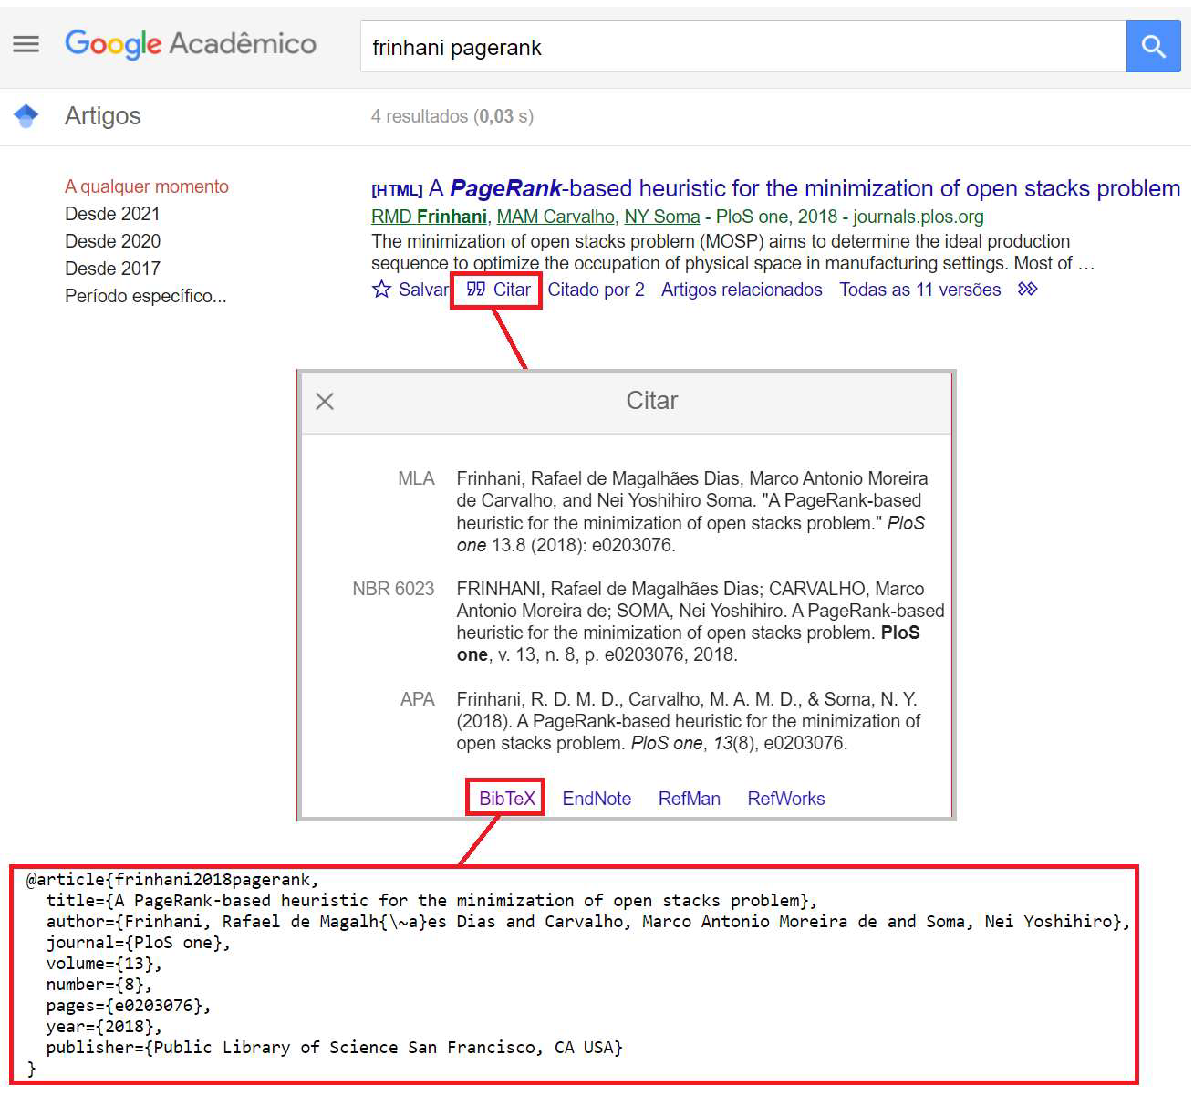
\includegraphics[width=0.48\textwidth]{figs/ref-GoogleAcademico.pdf}
\caption{Passos para obter referências \LaTeX~ pelo Google Acadêmico.}
\label{fig-PassosReferencia}
\end{figure}

Para mais informações sobre os campos exigidos em cada tipo de referência em \LaTeX acesse: \url{http://paginapessoal.utfpr.edu.br/jamhour/publicacoes/arquivos/00_Compilado_JabRef_dez2015.pdf}  